% xetex compatible variant that support TTF fonts according to company rules
\documentclass[ignorenonframetext, professionalfonts, hyperref={unicode}]{beamer}

\usetheme{Epam}

\usepackage{fontspec}
\setsansfont{SourceSansPro-Regular}
%\setbeamerfont{frametitle}{family=\fontspec{Oswald}}
\setbeamerfont{frametitle}{family=\fontspec{Oswald}}
\setbeamerfont{block title}{family=\fontspec{Oswald}}

%\setmainfont{Times New Roman}
\defaultfontfeatures{Mapping=tex-text}
\defaultfontfeatures{Ligatures=TeX}

%\setsansfont{Arial}
%\setromanfont{Trebuchet MS}

\usepackage{cmap}
\usepackage{graphicx}

\usepackage{textcomp}

\usepackage{beamerthemesplit}

\usepackage{ulem}

\usepackage{verbatim}
\usepackage{import}

\usepackage{listings}
\lstloadlanguages{bash}

\lstset{escapechar=`,
	captionpos=b,
	extendedchars=false,
	language=sh,
%	frame=single,
	tabsize=2, 
	columns=fullflexible, 
%	basicstyle=\scriptsize,
	keywordstyle=\color{blue}, 
	commentstyle=\itshape\color{brown},
%	identifierstyle=\ttfamily, 
	stringstyle=\mdseries\color{green}, 
	showstringspaces=false, 
	numbers=left, 
	numberstyle=\footnotesize, 
	breaklines=true, 
	inputencoding=utf8,
	keepspaces=true,
	morekeywords={u\_short, u\_char, u\_long, in\_addr}
	}

\definecolor{darkgreen}{cmyk}{0.7, 0, 1, 0.5}

\lstdefinelanguage{diff}
{
    morekeywords={+, -},
    sensitive=false,
    morecomment=[l]{//},
    morecomment=[s]{/*}{*/},
    morecomment=[l][\color{darkgreen}]{+},
    morecomment=[l][\color{red}]{-},
    morestring=[b]",
}

\author[Epam]{{\bf Epam}\\Low Level Programming Department}

%\institution[EPAM]{EPAM}
%\logo{\includegraphics[width=1cm]{logo.png}}

\graphicspath{{../../slides/cmdline/clipart/}{../../slides/bash/clipart/}}

\bibliographystyle{unsrt}
\setbeamertemplate{bibliography item}{\insertbiblabel}

\AtBeginSection[]{%
  \begin{frame}<beamer>
    \frametitle{}
    \tableofcontents[
        sectionstyle=show/shaded, hideallsubsections ]
  \end{frame}
  \addtocounter{framenumber}{-1}% If you don't want them to affect the slide number
}

% \regex for regular expressions
\newcommand{\regex}[1]{ %
\expandafter{$\ulcorner{\color{blue}\texttt{#1}}\lrcorner$} %
}


\title[bash]{Bourne again shell}

%%%%%%%%%%%%%%%%%%%%%%%%%%%%%%%%%%%%%%%%%%%%%%%%%
%%%%%%%%%% Begin Document  %%%%%%%%%%%%%%%%%%%%%%
%%%%%%%%%%%%%%%%%%%%%%%%%%%%%%%%%%%%%%%%%%%%%%%%%

\begin{document}

\begin{frame}
	\frametitle{BASH}
	\titlepage
	\vspace{-0.5cm}
	\begin{center}
	%\frontpagelogo
	\end{center}
\end{frame}

\begin{frame}
	\tableofcontents
%	[hideallsubsections]
\end{frame}



%%%%%%%%%%%%%%%%%%%%%%%%%%%%%%%%%%%%%%%%%   
%%%%%%%%%% Content starts here %%%%%%%%%%
%%%%%%%%%%%%%%%%%%%%%%%%%%%%%%%%%%%%%%%%%

%\section{Change execution flow with conditional command.}

% move this section to presentation 4
\section{Tests and conditions}
%\mode<all>{\begin{frame}[fragile]
    \frametitle{ Задание. Выполнить команды.}
\begin{block}{AND}
	\small\begin{lstlisting}
false && echo Not running
true && echo Running
	\end{lstlisting}
\end{block}

\begin{block}{OR}
	\small\begin{lstlisting}
false || echo Running
true || echo Not running
	\end{lstlisting}
\end{block}
\end{frame}
}
%\mode<all>{\begin{frame}[fragile]
    \frametitle{Общий синтаксис}

	\begin{block}{Конструкции для сравнения}
		\begin{itemize}
			\item {\tt \&\&} -- выполнится в случае успеха
			\item {\tt ||} -- выполнится в случае неудачи
		\end{itemize}
	\end{block}

	\begin{verbatim}
команда1 && команда2  или  условие1 && команда2 
команда1 || команда2  или  условие1 || команда2 
команда1 && команда2 && команда3 && ... && командаN
	\end{verbatim}

\end{frame}
}
% example && || chain
\mode<all>{\begin{frame}[fragile]{Условный оператор.}

Во время выполнения программы условный оператор позволяет выполнять разные наборы команд в зависимость от условного выражения.
\begin{columns}
  \column{0.6\textwidth}

В bash условное выражение - любая \alert{команда}. \\

Код возврата доступен через переменную \alert{\$?} \\

Поддерживает синтаксические конструкции: \alert{\&\&}, \alert{||}, \alert{if then (else)}, \alert{case}, \alert{select}.
А также cемейство команд для сравнения \alert{test}.

\column{0.4\textwidth}
\center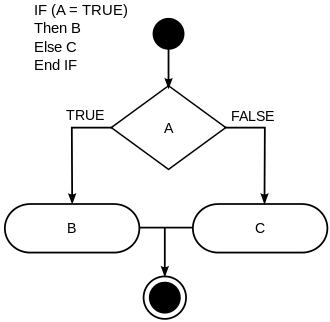
\includegraphics[width=4cm]{If-Then-Else-diagram}

 \end{columns}
    
\end{frame}
}
\mode<all>{\begin{frame}[fragile]
\frametitle{Условные операторы \&\& ||}

\underline{Выполнить команды:}
\begin{lstlisting}[language=bash]
 cd video && echo  Exit code $? Is OK. I am watching video.
 mkdir video # запустить предыдущую команду еще раз
\end{lstlisting}

\pause

Синтаксис:
\begin{verbatim}
command1 && command2
\end{verbatim}
Oболочка выполняет command2 если \alert{успешно} выполнилась command1. Логическая операция И (AND)
\pause

\underline{Выполнить команды:}
\pause
\begin{lstlisting}[language=bash]
cd video || echo Exit code $?. Video is not available 
rmdir video # Удалим и повторим еще раз первую команду.
\end{lstlisting}

\pause

Синтаксис:
\begin{verbatim}
command1 || command2
\end{verbatim}
Oболочка выполняет command2 если выполнилась c \alert{ошибкой} command1. Логическая операция ИЛИ (OR)
\end{frame}

}
\mode<all>{\begin{frame}[fragile]
\frametitle{Управляющие операторы}
Можно делать цепочки команд:
\begin{verbatim}
command1 && command2 || command3 
command1 && command2 && command3 && ...
\end{verbatim}

Применение операторов \&\& и ||:
\begin{itemize}
    \item Изменяют поведение кода в зависимости от успешности выполнения команд
    \item Объединяют команды
    \item Улучшают читаемость кода для простых проверок.  Одна строка vs три в if
    \item Но длинные цепочки сложно отлаживать и поддерживать
\end{itemize}

\end{frame}
}
% Команды сравнения.
\mode<all>{\begin{frame}[fragile]
   \frametitle{Команды сравнения.}

\underline{Выполнить команды:}
	\small\begin{lstlisting}
type -a test [ [[
test -f /etc/ ; echo $? # существует ли файл?
test -d /etc/ ; echo $? # существует ли директория?
	\end{lstlisting}

\pause
\alert{Команда test} сравнивают аргументы в условии. Если условие выполенено успешно, команда возвращет exit code \alert{0} иначе \alert{1}.

Синтаксис:
\begin{verbatim}
test expression 
[expression] 
[[ expression ]]
\end{verbatim}
expression - условное выражение. Синтаксис условного выражения может различаться от типа команды.
Есть несколько типов команд:

\begin{itemize}
    \item встроенные в оболочку test, [
    \item внешние /usr/bin/test, /usr/bin/[
    \item ключевое слово [[
\end{itemize}


\end{frame}
}

\mode<all>{\begin{frame}[fragile]
\frametitle{Что можно сравнивать в условии}

\underline{Выполнить команды:}
	\small\begin{lstlisting}
help test ; help [ ; help [[ # показывает опции для встроенных команды из оболочки
man test  # для внешней команды
\end{lstlisting}
    \pause
	\begin{itemize}
	    \item \alert{!} -- отрицание
	    \item \alert{-z} СТРОКА
	    \item СТРОКА1 \alert{==} СТРОКА2 или СТРОКА1 \alert{=} СТРОКА2
	    \item СТРОКА1 \alert{!=} СТРОКА2
	    \item ЦЕЛОЕ1 \alert{-eq} ЦЕЛОЕ2
	    \item ЦЕЛОЕ1 \alert{-ge} ЦЕЛОЕ2
	    \item ЦЕЛОЕ1 \alert{-lt} ЦЕЛОЕ2
	    \item \alert{-d} ФАЙЛ
	    \item \alert{-e} ФАЙЛ
	    \item \alert{-f} ФАЙЛ
	\end{itemize}

\end{frame}
}
%\mode<all>{\begin{frame}
    \frametitle{Условное выражение}
		\begin{itemize}
			\item Exit status любой программы
			\item Команда test или $[$ ... $]$
			\item $[[$ ... $]]$
			\item Двойные скобки {\bf (( ... ))} и конструкция {\bf let}
		\end{itemize}
\end{frame}
}


%% test and [[ comparison
\mode<all>{\begin{frame}[fragile]
    \frametitle{ Особенности использования [[ }
    \begin{block}{Кавычки обрабатываются по разному}
	\small\begin{lstlisting}
a="a b c" b="a b c"
[ $a = $b ] && echo $? # ошибка bash: [: too many arguments
[[ $a = $b ]] && echo $? # не нужно брать в кавычки ""
	\end{lstlisting}
    \end{block}

    \begin{block}{ Операторы \&\& AND || OR }
	\small\begin{lstlisting}
[[ "abc" = 1 -a "b" = 2 ]] # syntax error in conditional expression
[[ "abc" = 1 && "b" = 2 ]] # вместо -a использовать &&, -o ||
	\end{lstlisting}
    \end{block}
\end{frame}
}
\mode<all>{\begin{frame}[fragile]
    \frametitle{ Сравнение по шаблону}
    \begin{block}{ Pattern matching}
	\small\begin{lstlisting}
a="a b c"
[[ $a = a* ]] ; echo $? # строка совпадает с паттерном
[[ $a = d* ]] ; echo $? # символа d нет в строке
[[ $a = "a*" ]] ; echo $? # кaвычки отменяют паттерн
[[ $a =~ "a*" ]] ; echo $? # регулярные выражения
\end{lstlisting}
    \end{block}
\end{frame}
}
\mode<all>{\begin{frame}[fragile]
	\frametitle{Двойные квадратные скобки [[}

\begin{itemize}
        \item работает только в оболочках bash, zsh, ksh. Команды [ и test доступны в оболочках POSIX.
        \item Ведет себя не как команда, а как ключевое слово
        \item Доступны дополнительные сравнения (на соответствие регулярному выражению) или шаблону
        \item Нет необходимости закавычивать переменные и экранировать скобки \(\)
        \item Внутри можно использовать логические связки \({\tt \&\&, \|, \langle, \rangle}\)
\end{itemize}

\end{frame}
}

\mode<all>{\begin{frame}[fragile]
\frametitle{Синтаксис {\bf if}}

	\begin{columns}
		\column{0.5\textwidth}
	
	\begin{lstlisting}[language=bash]
if command1
then
    OTHER COMMANDS
elif command2
then
    OTHER COMMANDS
else
    OTHER COMMANDS
fi
\end{lstlisting}
		\column{0.5\textwidth}
Варианты форматирования
then отдельной строкой
	\begin{lstlisting}[language=bash]
if command
then OTHER COMMANDS 
fi
\end{lstlisting}

then и if на одной строке
	\begin{lstlisting}[language=bash]
if command; then 
    OTHER COMMANDS
fi
\end{lstlisting}
	\end{columns}

В зависимости от результата выполнения (exit code) command1 выполняется блок команд после then.   

Ключевое слово fi - обязательно

%	\pause
%	{\bf Практическое задание:} \\
%	\begin{itemize}
%
%		\item с помощью конструкции {\bf if} проверить существует ли файловый объект передаваемый в качестве параметра скрипту ({\tt man test})
%		\item если нет, то создать директорию с таким именем
%		\item если cуществует и файл является shell-скриптом ({\tt man file}), то запустить его
%		\item если существует и является директорией, то вывести на экран Top5 по размеру файлов из этой директории, 
%		    отсортированных в порядке убывания ({\tt man ls, man head})
%%	\end{itemize}
%	\end{columns}
\end{frame}
}
\mode<all>{\begin{frame}[fragile]
\frametitle{Условные операторы: case}

	\small
	\begin{columns}
		\column{0.3\textwidth}

		\begin{lstlisting}[language=sh,frame=single]
case "$variable" in 
 pattern1) command1
           command2
          ;;
 pattern2|pattern3)
         command3
         command4
        ;;
esac
\end{lstlisting}
		\pause

		\column{0.6\textwidth}
		{\normalsize Пример:}

		\begin{lstlisting}[language=bash]
#!/bin/bash

cmd=$1; var=$2
case "$cmd" in 
  --print|--echo)
    echo "Ура, печатаем!" ;;
  abc*|xyz*)
    echo "Странная команда $cmd" ;;
  *)
    echo "Я таких команд не знаю: $cmd" 1>&2
    exit 1 ;;
esac
[ ! -z "$var" ] && echo "переменная \$var=$var"
exit 0
\end{lstlisting}


	\end{columns}
\end{frame}
}
%\mode<all>{\begin{frame}[fragile]
\frametitle{case + getopt}
	Внешняя команда для обработки аргументов командной строки.
	\small
	\begin{lstlisting}
SHORTOPTS="af:h"
LONGOPTS="flagA,file:,help"
OPTS=$(getopt -o "$SHORTOPTS" -l "$LONGOPTS" -- "$@")

eval set -- "$OPTS" #  устанавливает $1 $2 ...

while [ $# -gt 0 ] ; do
  case $1 in
    -a|--flagA) FLAGA=$1 ; shift ;;
    -f|--file) FILE=$1; FILENAME="$2"; shift 2 ;;
    -h|--help) echo "Usage:$0 [-a|--flagA] [-h|--help] [-f|--file <filename>]"; exit 0;;
    --) shift; break ;; # skip this one
    *) ;;
  esac
done
\end{lstlisting}
\end{frame}
}
\mode<all>{\begin{frame}[fragile]
	\frametitle{case + getopts}
	
	Встроенная в bash обработка командной строки.

\begin{lstlisting}[language=sh,frame=single]
while getopts "af:h" Option
do
  case $Option in 
    a) FLAGA=1 ;;
    f) FILE=1
       FILENAME=$OPTARG
       ;;
    h) echo "Usage: $0 [-ah] -f <filename>";;
  esac  
done
shift $((OPTIND-1))
\end{lstlisting}
\end{frame}
}
%\mode<all>{\begin{frame}
\frametitle{Домашнее задание}

	Написать скрипт, который будет создавать файл, 
	записывать туда текущее время и переданную строку,
	используя при этом следующие аргументы командной строки: 

	\begin{enumerate}
		\item -f или -{}-file <имя файла>\\
			если отсутствует имя файла, то выйти с соответствующим сообщением;
		\item -l или -{}-log <строка>\\
			если отсутствует <строка>, то выйти с соответствующим сообщением;
		\item -a или -{}-append \\
			необязательный флаг, указывающий будет ли файл переписан, либо дописан.
	\end{enumerate}

	Cкрипт должен обрабатывать переданные аргументы с использованием {\tt getopt} либо {\tt getopts}.

\end{frame}
}
\mode<all>{\begin{frame}[fragile]
\frametitle{Условные операторы: select}

	\small
	\begin{columns}
		\column{0.3\textwidth}

		\begin{lstlisting}[language=sh,frame=single]
select variable [in list]
do
  command...
  break
done 
\end{lstlisting}
		\pause
		\column{0.7\textwidth}
		{\normalsize Пример:}

         \lstinputlisting[language=bash]{../../slides/bash/samples/select.sh}
		\pause
		\center{Удалить в select все [in *] и посмотреть на результат работы.}

	\end{columns}
\end{frame}
}

\section{Repeat operations with loops.}
\mode<all>{\begin{frame}
\frametitle{Основные конструкции для циклов}
  \begin{itemize}
   \item for - цикл просмотра (foreach), цикл со счетчиком 
   \item while, until - цикл с предусловием  
   \item break, continue  - досрочный выход, пропуск итерации
  \end{itemize}
\end{frame}
}
\mode<all>{\begin{frame}[fragile]
  \frametitle{Циклы for}
  \begin{enumerate}
    \item Стандартная форма
\begin{lstlisting}[language=sh,frame=single]
  for x in list 
  do
    op1
    op2
  done
\end{lstlisting}
    \item Арифметическая форма
\begin{lstlisting}[language=sh,frame=single]
  for (( expr1 ; expr2 ; expr3 )) 
  do 
    op1
    op2
  done
\end{lstlisting}
  \end{enumerate}
\end{frame}
}
\mode<all>{\begin{frame}[fragile]
\frametitle{ Циклы for. Примеры.}
  \begin{block}{Действие над файлами.}
\begin{lstlisting}[language=sh,frame=single]
for file in *
 do md5sum $file
done
\end{lstlisting}
  \end{block}

\begin{block}{Перечисление элементов.}
\begin{lstlisting}[language=sh,frame=single]
for planet in Mars Earth Mercury Saturn
 do echo $planet 
done
\end{lstlisting}
  \end{block}
\end{frame}
}
\mode<all>{\begin{frame}[fragile]
\frametitle{Циклы for. Цифровая последовательность.}
  \begin{block}{Примеры генерации.}
\begin{lstlisting}[language=bash,frame=single]
for num in 1 2 3 4 5 6 7 8 9 10 # простое перечисление 
 do ping 192.168.10.$num
done

for num in $(seq 1 10)  # генерация из внешней команды
 do ping 192.168.10.$num
done

for num in {1..10}  # генерация встроенными средствами
 do ping 192.168.10.$num
done

\end{lstlisting}
  \end{block}
\end{frame}
}
\mode<all>{\begin{frame}[fragile]
\frametitle{Циклы for. Цифровая последовательность.}
  \begin{block}{Арифметический формат (C-like) }
\begin{lstlisting}[language=bash,frame=single]
for ((i=1;i<11;i++))
do 
  echo $i
done  
\end{lstlisting}
  \end{block}

  \begin{block}{Несколько переменных}
    \begin{lstlisting}[language=sh,frame=single]
for ((a=1, b=1; a <= LIMIT ; a++, b++))
do
  echo -n "$a-$b"
done
\end{lstlisting}
  \end{block}
\end{frame}
}
\mode<all>{\begin{frame}[fragile]
\frametitle{ Циклы for. Примеры.}
  \begin{block}{Пустые выражения. Результат по умолчанию 1. }
    \begin{lstlisting}[language=sh,frame=single]
for (( i=1; ; i++))
do
  echo $i 
  [ "$i" -eq 10 ] && break 
done
    \end{lstlisting}
  \end{block}
\end{frame}
}
\mode<all>{\begin{frame}[fragile]
\frametitle{ Цикл for. Примеры.}
  \begin{block}{Aргументы командной строки.}
    \begin{lstlisting}[language=bash,frame=single]
for arg
 do echo $arg 
done
    \end{lstlisting}
  \end{block}
  \begin{block}{Из переменной. Запись одной строкой.}
    \begin{lstlisting}[language=bash,frame=single]
for name in "$users" ; do echo $name ; done
    \end{lstlisting}
  \end{block}
\end{frame}
}
% while
\mode<all>{\begin{frame}[fragile]
\frametitle{Циклы while,until}
\begin{lstlisting}[language=sh,frame=single]
while expr1; ... exprN
do
 op
done
\end{lstlisting}
Применяются когда нужно повторять до выполнения какого-то события, когда количество элементов неизвестно заранее. Например oкончание файла, ввод текста пользователем, ожидание хоста в сети после презагрузки. 
\end{frame}
}
\mode<all>{\begin{frame}[fragile]
\frametitle{Примеры использования while}

\begin{block}{Перебираем аргументы.}
\begin{lstlisting}[language=bash,frame=single]
while [[ -n $1 ]]
do
    echo $1
    shift # rename the positional parameters $N+1,$N+2 ... to $1,$2 (N=1)
done
\end{lstlisting}
\end{block}

%\begin{block}{Пример. Перебираем аргументы.}
%\lstinputlisting[language=bash,frame=single]{../../slides/bash/samples/while_args.sh}
%\end{block}
\end{frame}

%\begin{block}{Пример. Несколько команд.}
%\begin{lstlisting}[language=sh,frame=single]
%while ((i++))
% read y
%do
% echo $i $y
% [[ "$y" = 'stop' ]] && break
%done
%\end{lstlisting}
%\end{block}

%\begin{frame}[fragile]
%\frametitle{Пример. Бесконечный цикл.}
%\begin{block}{Выход из бесконечного цикла.}
%\begin{lstlisting}[language=bash,frame=single,name=random.sh]
%while :
%do
%  x=$RANDOM
%  echo $x
%  [[ $x -gt 1100 ]] && break
%done
%\end{lstlisting}
%\end{block}
%\end{frame}
}
\mode<all>{\begin{frame}[fragile]
\frametitle{ Цикл until. Пример.}
  \begin{block}{Ожидаем хост после перезагрузки.}
    \begin{lstlisting}[language=sh,frame=single]
until ping -q -c 3  $host 1>/dev/null 2>&1 && nc -z $host 22
do 
   sleep 1
   echo unavailable;
done
\end{lstlisting}
  \end{block}
\end{frame}
}
\mode<all>{\begin{frame}[fragile]
\frametitle{Перенаправление из цикла.}
  \begin{block}{Pipe}
    \begin{lstlisting}[language=sh,frame=single]
for name in $users ; do echo $name ; done | wc -l
    \end{lstlisting}
  \end{block}
  \begin{block}{В файл}
    \begin{lstlisting}[language=sh,frame=single]
for name in $users ; do echo $name ; done
(( i=10 )); while (( i > 0 )); do 
    echo "$i"
    (( i-- ))
done > output.txt
    \end{lstlisting}
  \end{block}
\end{frame}
}
\mode<all>{\begin{frame}[fragile]
\frametitle{Перенаправление из цикла.}

  \begin{block}{Парсер.}
    \begin{lstlisting}[language=sh,frame=single]
while IFS=":" read name pass uid guid comment home shell ; do
    echo $name $uid $guid $home $shell 
done < /etc/passwd
    \end{lstlisting}
  \end{block}

  \begin{block}{Построчное чтение из файла.}
    \begin{lstlisting}[language=sh,frame=single]
while IFS= read -r line; do
  printf '%s\n' "$line"
done < "$file"
    \end{lstlisting}
  \end{block}
\end{frame}
}
\mode<all>{\begin{frame}[fragile]
\frametitle{Внешние команды.}
Массовые операции с файлами аналог циклов
  \begin{block}{Команда find}
    \begin{lstlisting}[language=sh,frame=single]
find . -name '*.c' -exec stat  {} \;
    \end{lstlisting}
  \end{block}
  \begin{block}{Команда xargs}
    \begin{lstlisting}[language=sh,frame=single]
echo /dev/std* | xargs -n1 readlink
    \end{lstlisting}
  \end{block}
\end{frame}
}
%\mode<all>{\begin{frame}[fragile]
    \frametitle{Упражнения}
    \begin{enumerate}
        \item Посчитать сумму кубов чисел от 1 до 100
        \item Вывести в файл 10 случайных чисел от 0 до 80
        \item Построить гистограмму данных из предыдущего файла файла {\bf Hint:} {\tt while read, echo -n }
    \end{enumerate}
\end{frame}
}
%
\section{Group pieces of code with functions.}
\mode<all>{\begin{frame}
	\frametitle{Функции}

	\begin{itemize}
		\item Именованные
		\item Неименованные
	\end{itemize}

	Функции в shell могут использоваться как обычные программы, которые:
	\begin{itemize}
		\item Принимают позиционные параметры;
		\item возвращают статус;
		\item Могут использоваться в качестве источника либо приемника 
			при перенаправлениях ввода/вывода.
	\end{itemize}

\end{frame}
}
\mode<all>{\begin{frame}[fragile]
	\frametitle{Функции: синтаксис}
	\begin{itemize}
		\item Классический синаксис c ключевым словом \alert{function}: 
                        \begin{lstlisting}[language=bash,frame=single]
function function_name {
  command...
}
\end{lstlisting}
		\item Портабельный (C-style):
			\begin{lstlisting}
function_name()
{
  command...
} 
\end{lstlisting}

		\item Однострочный:
                        \begin{lstlisting}[language=bash,frame=single]
function_name () { command... ;}
\end{lstlisting}
  \end{itemize}
\end{frame}
}
%\mode<all>{\begin{frame}[fragile]
	\frametitle{Пример: shellshock}
	\begin{block}{Однострочный синтаксис}
			\begin{lstlisting}
function_name () { command... ;}
\end{lstlisting}
	\end{block}

    В 2014 году вскрылась уязвимость, существовавшая с {\bf 1992} г.:

	\begin{block}{Shellshock}
			\begin{lstlisting}
export badvar='(){:;}; echo "The Matrix has you"'
bash -c "echo Just a simple shell call"
\end{lstlisting}
	\begin{itemize}
	    \item Объявление переменной
	    \item Создание процесса, наследующего опасную переменную
	    \item При инициализации окружения {\tt bash} запускает на выполнение все, что следует за ``объявлением'' функции
	\end{itemize}
	\end{block}

\end{frame}
}
% example
\mode<all>{\begin{frame}[fragile]
	\frametitle{Пример (начало)}
	\small
        \begin{lstlisting}[language=bash,frame=single]
#!/bin/bash

function help {
  echo "Использование: $0 <string>"
  exit 1
}

f1(){
  echo Вызвана функция $FUNCNAME с $# аргументами
}

f2(){
  while read str; do
    echo ${FUNCNAME}: прочитана строка: $str
  done
}
\end{lstlisting}

\end{frame}
}
\mode<all>{\begin{frame}[fragile]
	\frametitle{Пример (окончание)}
	\small
	\begin{lstlisting}
[ $# -eq 0 ] && help

f1 "$@"

{ for ((i=0;i<5;i++));do
  echo $@
done } | f2

exit
\end{lstlisting}

\end{frame}
}
\mode<all>{\begin{frame}[fragile]
	\frametitle{Локальные переменные}

	Переменные объявленные с префиксом {\tt local} видны только внутри объявленного блока.

	\small
	\begin{columns}
		\column{0.5\textwidth}
        \begin{lstlisting}[language=bash,frame=single]
#!/bin/bash

VAR=test
f1(){
  local VAR=test1
  echo Function ${FUNCNAME}: VAR=$VAR
}
f2(){
  VAR=test2
  echo Function ${FUNCNAME}: VAR=$VAR
}
\end{lstlisting}
		\column{0.5\textwidth}	
\begin{lstlisting}[language=bash,frame=single]
echo Before f1: VAR=$VAR
f1
echo Before f2: VAR=$VAR
f2
echo After f2: VAR=$VAR

exit
\end{lstlisting}
	\end{columns}

\end{frame}
}
%\mode<all>{\begin{frame}
	\frametitle{Домашнее задание}
	\begin{itemize}
		\item Создать библиотеку функций:
			\begin{itemize}
				\item функция {\tt help};
				\item функция {\tt count\_str} -- подсчитывает количество найденных строк в stdin.
				\item функция {\tt readfile}, в которую передается имя файла в качестве 1 параметра
					и строка, которую необходимо найти, в качестве 2-го.
					Задача функции -- вырезать из файла все пустые строки и комментарии, 
					и с помощью предыдущей функции вернуть количество вхождений искомой строки.
			\end{itemize}
		\item Создать скрипт, который обрабатывает файл переданный через параметр -f или -{}-file;
		\item Включить библиотеку в свой скрипт с помощью {\tt source};
		\item Найти количество сервисов {\tt tcp} в файле {\tt /etc/services};
		\item Найти количество сервисов {\tt udp} в файле {\tt /etc/services};
  \end{itemize}
\end{frame}
}

\section{Debugging scripts.}
\mode<all>{\begin{frame}[fragile,allowframebreaks]
	\frametitle{Включение режима отладки}
	Используется команда {\tt set} для активизации различных режимов работы {\tt bash}.

	Включение режима производится с помощью ''-'',\\
	а отключение -- ''+''.

	\begin{block}{Примеры включения режима отладки.}
		\begin{lstlisting}[language=sh]
bash -x ./script.sh # опция командной строки

#!/bin/bash -x # внутри скрипта опцией
[.. script ..]

#!/usr/bin/env bash
set -x # внутри скрипта командой 

#!/usr/bin/env bash
[..irrelevant code..]
set -x  # включаем отладку на часть кода
[..relevant code..]  
set +x # выключаем отладку
[..irrelevant code..]
		\end{lstlisting}
	\end{block}
\end{frame}
}
\mode<all>{\begin{frame}[fragile,allowframebreaks]
	\frametitle{Ключи отладки команды set}

	\begin{itemize}
		\item {\tt set -v} -- вывод на экран исполняемой строки
			\begin{lstlisting}[language=sh]
set -v
echo $HOME
			\end{lstlisting}

		\item {\tt set -x} -- вывод на экран исполняемой строки с автоматической подстановкой значений переменных
\begin{lstlisting}[language=sh]
set -x
echo $HOME
\end{lstlisting}

		\item {\tt set -n} -- проверка синтаксиса скрипта
\begin{lstlisting}[language=sh]
bash -n test.sh
\end{lstlisting} 


		\item {\tt set -f} -- отключение генерации имен файлов с использованием метасимволов (globbing)
\begin{lstlisting}[language=sh]
echo ~/.*
set -f
echo ~/.*
\end{lstlisting} 
		\framebreak
		\item {\tt set -e} -- остановка выполнения скрипта, если какая-либо команда 
		возвращяет errorstatus не равный 0
			\begin{lstlisting}[language=sh]
#!/bin/bash

set -e
false || true
echo Working
false
echo Still working
			\end{lstlisting} 
	\end{itemize}
\end{frame}
}
% debug variables
\mode<all>{\begin{frame}[fragile]
	\frametitle{Отладочные переменные}

  \begin{tabular}{ l  p{7cm} }
    \alert{\$LINENO}  & номер текущей строки \\ 
    \alert{\$FUNCNAME} & массив содержит имена всех функций из стека вызовов. 0 элемент\, имя текущей функции \\
    \alert{\$BASH\_SOURCE} & массив\, содержит имена подключенных файлов source\\
    \alert{\$SHLVL} & уровень вложенности интерпретатора \\
    \alert{\$PIPESTATUS} & массив статусов завершения всех команд в pipe \\
    \end{tabular}

	\begin{block}{Альтернативный вид PS4.}
		\begin{lstlisting}[language=sh]
export PS4='+(${BASH_SOURCE}:${LINENO}): ${FUNCNAME[0]:+${FUNCNAME[0]}(): }'
		\end{lstlisting}
	\end{block}
\end{frame}
}
\mode<all>{\begin{frame}[fragile]
	\frametitle{Стек вызовов}

	\begin{itemize}
		\item {\tt caller [N]} -- функция выводит на экран номер строки, имена функции и файла вызывающего скрипта
	\end{itemize}

	\begin{block}{backtrace}
		\begin{lstlisting}[language=sh]
#!/bin/bash
backtrace() {
  echo Backtrace:
  for((i=$SHLVL;i>=0;i--)); do
    caller $i
  done
}
f1() {
  echo Function $FUNCNAME at $LINENO && backtrace
}
f1
		\end{lstlisting}
	\end{block}

\end{frame}
}
% TODO 2 things in one. typical errors in conditions
% directory script   filetype file
% ./filetype 
% ./filetype "file 1"
%common conditional operator errors
\mode<all>{\begin{frame}[fragile]
\frametitle{Типичные ошибки в условном выражении}

	Написать скрипт прнимающий один аргумент и определяющий файл ли это. Если файл выводить на экран строку 'regular file detected' в случае успеха,
Предварительно создать: файлы c именами file, my file
	\begin{block}{check.sh - исправить}
      \lstinputlisting[firstline=3, lastline=12,language=bash]{../../slides/bash/samples/check.sh}
    \end{block}
    \normalsize
	И запустить этот скрипт:
	
	\begin{enumerate}
            \item {\tt ./check.sh file} 
            \item {\tt ./check.sh "my file" \# параметр с пробелом}
            \item {\tt ./check.sh \# без параметров}
        \end{enumerate}

\end{frame}
}
%\mode<all>{\begin{frame}
	\frametitle{Пример: варианты исправления}

		\begin{enumerate}
			\item {\tt [ ``\$STRING'' == ``\$VAR'' ] }
			\item {\tt [ z\$STRING == z\$VAR ] }
		\end{enumerate}

\end{frame}
}
\mode<all>{\begin{frame}[fragile]
	\frametitle{Сообщения об ошибках}

	\begin{block}{Пример.}
		\begin{lstlisting}[language=sh]
bash: test: too many arguments

script.sh: line 100: syntax error: unexpected end of file

script.sh: line 50: unexpected EOF while looking for matching `"' 


		\end{lstlisting}
	\end{block}

\end{frame}
}

\end{document}
